\chapter{Исследовательский раздел}
\section{Технические характеристики}
Технические характеристики устройства, на котором выполнялись исследования разработанного метода:

\begin{itemize}
	\item[---] операционная система Window 10 Home Single Language \cite{window};
	\item[---] память 8 Гб;
	\item[---] процессор 11th Gen Intel(R) Core(TM) i5-1135G7 2.42 ГГц, 4 ядра \cite{cpu}.
\end{itemize}

Во время выполнения исследований устройство было подключено к сети электропитания, нагружено приложениями окружения и самой системой замера.

Для проведения исследований разработанного метода используются выборки, созданные на основе текстов по 5 темам: Наука и техника, Спорт, Культура, Экономика и Мир. Количество текста по каждой тематике в каждой выборке используется одинаковое. Исходная выборка разбивается на обучающую (80\% объема) и тестовую (20\%) выборки. 

Как отмечалось раньше, метрики аккуратности и F1-меры используются в качестве метрики для оценки качества классификатора.

\section{Влияние размера обучающей выборки}
Обучающая выборка --- это набор данных, который используется для обучения модели машинного обучения. Она представляет собой подмножество общего набора данных, которое содержит примеры, сопоставленные с соответствующими целевыми значениями или метками. Размер обучающей выборки --- фактор, влияющий на качество классификатора.

Для проведения данного исследования было проведено сравнение зависимости времени обучения и качества классификатора от количества текстов на обучающей выборке.

Результаты проведенного исследования приведены в таблицах \ref{tab:4.1_a} и \ref{tab:4.1_b}.

\begin{table}[H]
	\centering
	\caption{Замеры времени обучения от размера выборки}\label{tab:4.1_a}
	\begin{tabular}{|T|T|T|}
		\hline
        \textit{Количество текстов в выборке} & \textit{Время обучения классификатора (с.)} \\ \hline
        50 & 0.03 \\ \hline
        100 & 0.08 \\ \hline
        200 & 0.23 \\ \hline
        500 & 1.59 \\ \hline
        1000 & 5.67 \\ \hline
        2000 & 21.29 \\ \hline
        3000 & 47.39 \\ \hline
        4000 & 82.76 \\ \hline
        5000 & 135.10 \\ \hline
	\end{tabular}
\end{table}

\begin{table}[H]
	\centering
	\caption{Зависимость качества классификатора от размера выборки}\label{tab:4.1_b}
	\begin{tabular}{|T|T|T|}
		\hline
        \textit{Количество текстов в выборке} & \textit{Точность на тестовой выборке} & \textit{F1-мера}\\ \hline
		50 & 0.2 & 0.27 \\ \hline
        100 & 0.9 & 0.89 \\ \hline
        200 & 0.9 & 0.90 \\ \hline
        500 & 0.91 & 0.92 \\ \hline
        1000 & 0.917 & 0.93\\ \hline
        2000 & 0.92 & 0.935 \\ \hline
        3000 & 0.94 & 0.937 \\ \hline
        4000 & 0.942 & 0.94 \\ \hline
        5000 & 0.943 & 0.943 \\ \hline
	\end{tabular}
\end{table}

Ниже, на рисунках \ref{img:4.1a} и \ref{img:4.1b}, представлены данные из таблиц \ref{tab:4.1_a} и \ref{tab:4.1_b} соответственно в виде графика.

\captionsetup{justification=centering,singlelinecheck=off}
\begin{figure}[h!]
	\centering
		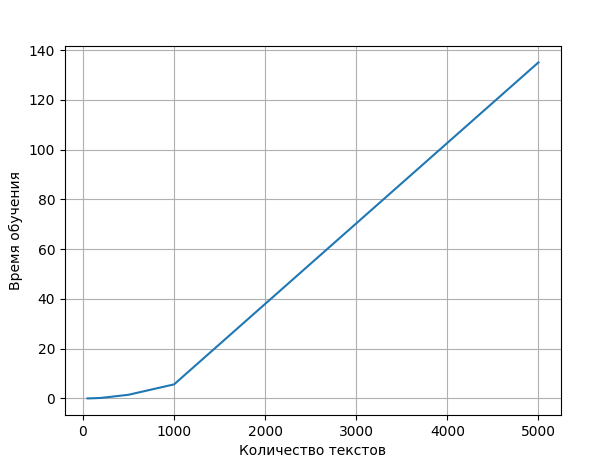
\includegraphics[,scale=0.9]{./img/4.1a.png}
		\caption{График зависимости времени обучения от размера выборки}  
		\label{img:4.1a}
\end{figure}

\captionsetup{justification=centering,singlelinecheck=off}
\begin{figure}[h!]
	\centering
		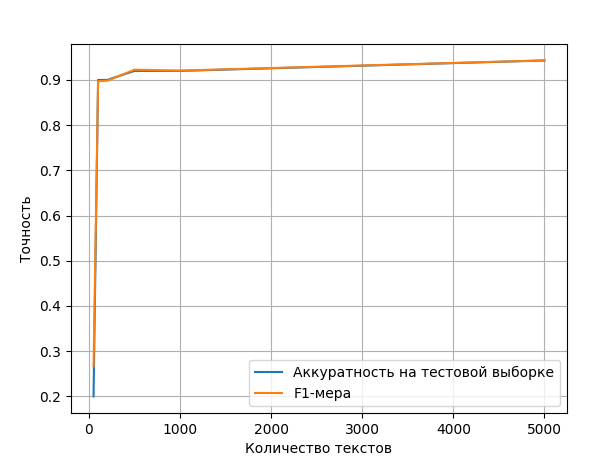
\includegraphics[,scale=0.85]{./img/4.1b.png}
		\caption{График зависимости качества классификатора от размера выборки}  
		\label{img:4.1b}
\end{figure}
\newpage

На основании полученных результатов можно сделать вывод, что количество текстов в обучающей выборке влияет на время обучения и качество классификатора. При использовании выборок с меньшим количеством текста классификатор будет обучаться за меньшее время, но с низкой точностью. По мере увеличения количества текстов в обучающей выборке точность классификатора также увеличивается. Стоит отметить, что увеличение количества текстов увеличивает время обучения, но существенно не увеличивает точность классификатора после того, как количество текстов достигнет 1000.

Таким образом, можно обучить классификатор на выборке из 1000 текстов для оптимизации времени обучения и качества классификатора.

\section{Влияние наличия стоп-слов в тексте}
На этапе предварительной обработки текста происходит процесс удаления стоп-слов. Как отмечалось ранее, стоп-слова --- это текстовые шумы или неинформативные слова, которые встречаются в большом количестве, но не имеют семантического значения и при игнорировании этих слов исходное предложение не теряет своего смысла.

Для проведения данного исследования было проведено сравнение зависимости качества классификатора от наличия процесса удаления стоп-слов на этапе предварительной обработки текстов.

Результаты проведенного исследования приведены в таблице \ref{tab:4.2}.

\begin{table}[H]
	\centering
	\caption{Зависимость качества классификатора от наличия стоп-слов}\label{tab:4.2}
	\begin{tabular}{|m{5em}|m{6.9em}|m{7em}|m{5.5em}|m{4.8em}|}
		\hline
        \textit{Количество текстов} & \textit{Точность на тестовой выборке (Без)} & \textit{Точность на тестовой выборке (С)} & \textit{F1-мера (Без)} & \textit{F1-мера (С)}\\ \hline
		50 & 0.2 & 0.2 & 0.27 &0.27 \\ \hline
        100 & 0.9 & 0.95 & 0.89 &0.94\\ \hline
        200 & 0.9 & 0.90 & 0.90 &0.90\\ \hline
        500 & 0.92 & 0.93 & 0.92 &0.93\\ \hline
        1000 & 0.92 & 0.91 & 0.92 &0.91\\ \hline
        5000 & 0.943 & 0.933 & 0.94 &0.93\\ \hline
	\end{tabular}
\end{table}

Ниже, на рисунках \ref{img:4.2a} и \ref{img:4.2b}, представлены данные из таблицы \ref{tab:4.2} в виде графика.

\captionsetup{justification=centering,singlelinecheck=off}
\begin{figure}[h!]
	\centering
		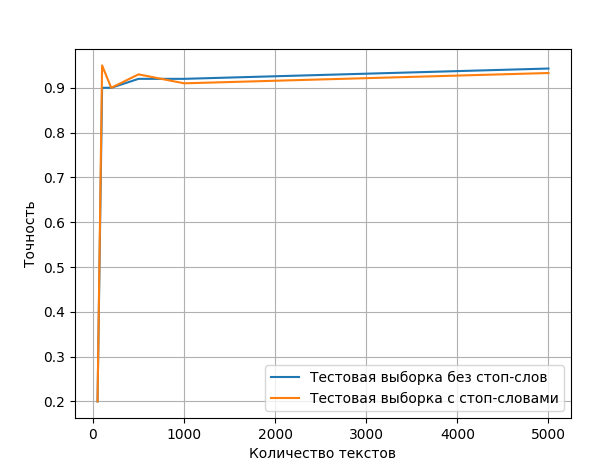
\includegraphics[,scale=0.85]{./img/4.2a.png}
		\caption{График зависимости точности классификатора от наличия стоп-слов}  
		\label{img:4.2a}
\end{figure}

\captionsetup{justification=centering,singlelinecheck=off}
\begin{figure}[h!]
	\centering
		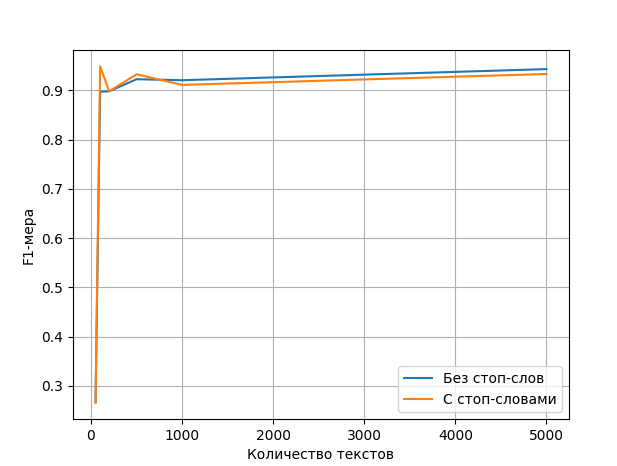
\includegraphics[,scale=0.9]{./img/4.2b.png}
		\caption{График зависимости F1-меры от наличия стоп-слов}  
		\label{img:4.2b}
\end{figure}
\newpage

На основании полученных результатов можно сделать вывод, что наличие стоп-слов в тексте обучающей выборки не сильно влияет на качество классификатора. В обучающих выборках с небольшим количеством текста (с 50 до 500 текстов) с стоп-словами обученные на них классификаторы имеют несколько более высокую точность, чем классификаторы, обученныы на обучающих выборках без стоп-слов (на 1-2\%). Но в обучающих выборках с большим количеством текстов (1000 или 5000 текстов) классификаторы, обученные на обучающих выборках без стоп-слов, имеют более высокую точность (на 1\%).

\section{Влияние ядра метода опорных векторов}
Ядро (kernel) в методе опорных векторов определяет функцию, которая вычисляет скалярное произведение двух векторов в пространстве признаков. Оно позволяет проецировать данные в более высокомерное пространство, где они могут быть линейно разделимыми, даже если исходное пространство не является линейно разделимым. 

Для проведения этого исследования было проведено сравнение зависимости качества классификатора от ядра метода опорных векторов при использовании следующих ядер: линейное, полиномиальное, Гауссово RBF и сигмоидальное.

Ниже, на рисунках \ref{img:4.3a} и \ref{img:4.3b}, представлены результаты проведенного исследования 
\captionsetup{justification=centering,singlelinecheck=off}
\begin{figure}[h!]
	\centering
		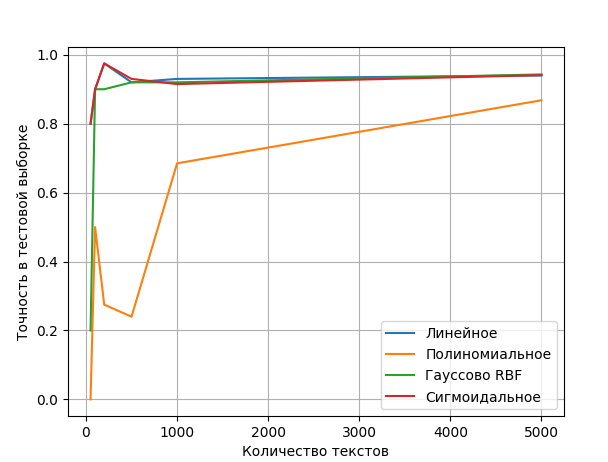
\includegraphics[,scale=0.9]{./img/4.3a.png}
		\caption{График зависимости точности классификатора от ядер}  
		\label{img:4.3a}
\end{figure}

\captionsetup{justification=centering,singlelinecheck=off}
\begin{figure}[h!]
	\centering
		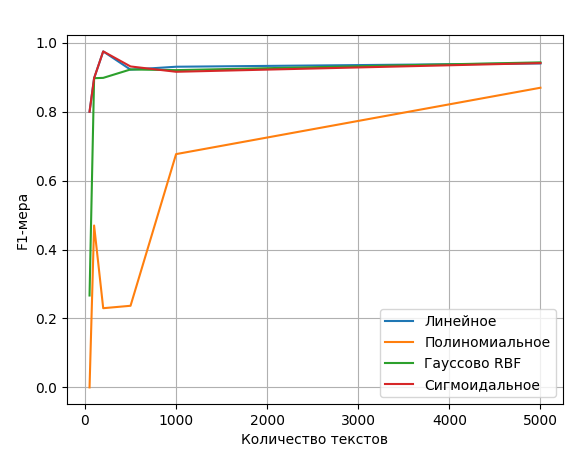
\includegraphics[,scale=0.9]{./img/4.3b.png}
		\caption{График зависимости F1-меры от ядер}  
		\label{img:4.3b}
\end{figure}
\newpage

Из полученных результатов можно сделать вывод, что зависимости точности и F1-меры классификатора от различных ядер совпадают. Классификатор с полиномиальным ядром имеет наименьшее качество, а классификаторы с другими ядрами имеет примерно одинаковую точность.

\section*{Вывод}
В этом разделе были описаны технические характеристики устройства для проведения исследований и приведены исследования разработанного метода. Из полученных результатов исследований можно сделать вывод, что при увеличении количества текстов в обучающей выборке время обучения классификатора будет быстро увеличиваться, но точность классификатора возрастает ненамного для обучающих выборок с большим количеством текстов. Результаты также показывают, что процесс удаления стоп-слов на этапе предварительной обработки текста не сильно влияет на качество классификатора. Использование различных ядер для классификатора показывает, что использование линейного ядра, гауссовского ядра RBF и сигмоидального ядра приводит к получению высокоточного классификатора.
